%%
%% This is file `sample-acmlarge.tex',
%% generated with the docstrip utility.
%%
%% The original source files were:
%%
%% samples.dtx  (with options: `acmlarge')
%% 
%% IMPORTANT NOTICE:
%% 
%% For the copyright see the source file.
%% 
%% Any modified versions of this file must be renamed
%% with new filenames distinct from sample-acmlarge.tex.
%% 
%% For distribution of the original source see the terms
%% for copying and modification in the file samples.dtx.
%% 
%% This generated file may be distributed as long as the
%% original source files, as listed above, are part of the
%% same distribution. (The sources need not necessarily be
%% in the same archive or directory.)
%%
%% The first command in your LaTeX source must be the \documentclass command.
\DeclareUnicodeCharacter{223C}{~}
\documentclass[acmlarge]{acmart}

%%
%% \BibTeX command to typeset BibTeX logo in the docs
\AtBeginDocument{%
  \providecommand\BibTeX{{%
    \normalfont B\kern-0.5em{\scshape i\kern-0.25em b}\kern-0.8em\TeX}}}

%% Rights management information.  This information is sent to you
%% when you complete the rights form.  These commands have SAMPLE
%% values in them; it is your responsibility as an author to replace
%% the commands and values with those provided to you when you
%% complete the rights form.
\setcopyright{acmcopyright}
\copyrightyear{2020}
\acmYear{2020}
\acmDOI{10.1145/1122445.1122456}


%%
%% These commands are for a JOURNAL article.
\acmJournal{IMWUT}
\acmVolume{0}
\acmNumber{0}
\acmArticle{0}
\acmMonth{0}

%%
%% Submission ID.
%% Use this when submitting an article to a sponsored event. You'll
%% receive a unique submission ID from the organizers
%% of the event, and this ID should be used as the parameter to this command.
%%\acmSubmissionID{123-A56-BU3}

%%
%% The majority of ACM publications use numbered citations and
%% references.  The command \citestyle{authoryear} switches to the
%% "author year" style.
%%
%% If you are preparing content for an event
%% sponsored by ACM SIGGRAPH, you must use the "author year" style of
%% citations and references.
%% Uncommenting
%% the next command will enable that style.
%%\citestyle{acmauthoryear}

%%
%% end of the preamble, start of the body of the document source.
\begin{document}

%%
%% The "title" command has an optional parameter,
%% allowing the author to define a "short title" to be used in page headers.
\title{GazeDance: A High Frame Rate Eye-tracking Framework Specialized for Mobile Device}

%%
%% The "author" command and its associated commands are used to define
%% the authors and their affiliations.
%% Of note is the shared affiliation of the first two authors, and the
%% "authornote" and "authornotemark" commands
%% used to denote shared contribution to the research.
% \author{Ben Trovato}
% \authornote{Both authors contributed equally to this research.}
% \email{trovato@corporation.com}
% \orcid{1234-5678-9012}
% \author{G.K.M. Tobin}
% \authornotemark[1]
% \email{webmaster@marysville-ohio.com}
% \affiliation{%
%   \institution{Institute for Clarity in Documentation}
%   \streetaddress{P.O. Box 1212}
%   \city{Dublin}
%   \state{Ohio}
%   \postcode{43017-6221}
% }

% \author{Lars Th{\o}rv{\"a}ld}
% \affiliation{%
%   \institution{The Th{\o}rv{\"a}ld Group}
%   \streetaddress{1 Th{\o}rv{\"a}ld Circle}
%   \city{Hekla}
%   \country{Iceland}}
% \email{larst@affiliation.org}

% \author{Valerie B\'eranger}
% \affiliation{%
%   \institution{Inria Paris-Rocquencourt}
%   \city{Rocquencourt}
%   \country{France}
% }

% \author{Aparna Patel}
% \affiliation{%
%  \institution{Rajiv Gandhi University}
%  \streetaddress{Rono-Hills}
%  \city{Doimukh}
%  \state{Arunachal Pradesh}
%  \country{India}}

% \author{Huifen Chan}
% \affiliation{%
%   \institution{Tsinghua University}
%   \streetaddress{30 Shuangqing Rd}
%   \city{Haidian Qu}
%   \state{Beijing Shi}
%   \country{China}}

% \author{Charles Palmer}
% \affiliation{%
%   \institution{Palmer Research Laboratories}
%   \streetaddress{8600 Datapoint Drive}
%   \city{San Antonio}
%   \state{Texas}
%   \postcode{78229}}
% \email{cpalmer@prl.com}

% \author{John Smith}
% \affiliation{\institution{The Th{\o}rv{\"a}ld Group}}
% \email{jsmith@affiliation.org}

% \author{Julius P. Kumquat}
% \affiliation{\institution{The Kumquat Consortium}}
% \email{jpkumquat@consortium.net}

%%
%% By default, the full list of authors will be used in the page
%% headers. Often, this list is too long, and will overlap
%% other information printed in the page headers. This command allows
%% the author to define a more concise list
%% of authors' names for this purpose.
% \renewcommand{\shortauthors}{Trovato and Tobin, et al.}

%%
%% The abstract is a short summary of the work to be presented in the
%% article.
\begin{abstract}
Gaze-on-screen tracking, an appearance-based eye-tracking task, has drawn significant interest in recent years. While learning-based high-precision eye-tracking methods have been designed in the past, the complex pre-training and high computation in neural networks restrict their applicability in mobile devices. Moreover, as the display frame rate of mobile devices has steadily increased to 120Hz, high-precision eye tracking becomes increasingly challenging. In this work, we tackle these challenges and introduce GazeDance, a biologic-inspired eye-tracking model specialized for mobile devices offering both high performance and efficiency. Specifically, we design a flexible suspending mechanism through the transformation of interaction state with two novel operations: "divide-and-rule" and inter-frame information sharing. Compared to existing methods, GazeDance achieves approximately 6× speedup and 15\% accuracy improvement on mobile devices. The efficacy of GazeDance is further demonstrated with real-world applications and an open-source development toolkit has been publicly released to support industry adoption. 

\end{abstract}

%%
%% The code below is generated by the tool at http://dl.acm.org/ccs.cfm.
%% Please copy and paste the code instead of the example below.
%%
\begin{CCSXML}
<ccs2012>
<concept>
<concept_id>10003120.10003138.10003140</concept_id>
<concept_desc>Human-centered computing~Ubiquitous and mobile computing systems and tools</concept_desc>
<concept_significance>300</concept_significance>
</concept>
</ccs2012>
\end{CCSXML}

   

\ccsdesc[300]{Human-centered computing~Ubiquitous and mobile computing systems and tools}

%%
%% Keywords. The author(s) should pick words that accurately describe
%% the work being presented. Separate the keywords with commas.
\keywords{mobile scenario, eye movement classification, gaze detection, convolutional neural network,  recurrent neural networks}


%%
%% This command processes the author and affiliation and title
%% information and builds the first part of the formatted document.
\maketitle

\section{Introduction}
%  Though model-based or appearance-based most solutions for gaze-on-screen tracking suffered from low accuracy because of the limited technology and the lack of large-scale data.
Eye-tracking has been an active research topic in the field of human-computer interaction with potential adoption across a wide range of psychological and medical applications, e.g., people with motor impairments~\cite{}. As mobile devices have become the de facto human-computer interface, recent work has been focusing on developing gaze-on-screen tracking technologies tackling mobile-specific design chal mobile e.g., delenges, vices. Mobile-specific design challenges include 

With the widespread use of mobile devices and the rising research interest of mobile human-computer interaction, more studies have focused directly on the user's gaze position on the screen of mobile devices. As a ubiquitous task, it distinguishes from the pure eye-tracking model for complex dynamic conditions such as the varying external light and different levels of jitter. We define this task as gaze-on-screen tracking in this work. 

Early solutions for gaze-on-screen tracking suffered from low accuracy because of the limited technology and the lack of large-scale data. With the heavy usage of cameras on cellphones in recent years, some large-scale datasets are available (e.g., GazeCapture \cite{krafka2016eye}), which makes a great contribution to the performance of gaze-on-screen models. While great progress has been made in gaze-on-screen tracking, it is still a challenging problem to put those models performed well under experimental settings on common mobile devices for the following reasons: (1) complex pre-training and enormous computation. Most of the existing models require high quality of hardware to satisfy the huge amount of computation, which is too expensive to be equipped in common smartphones. For example, the number of layers of ResNet \cite{he2016deep} and DenseNet \cite{huang2017densely} can be up to one thousand; (2)jitter adaptability. A large portion of mobile human-computer interaction is based on handheld mobile devices in a variety of scenarios such as walking and taking the subway, leading to jitter playing an inevitable and unneglectable role during interactions. However, most current methods can not well generalize the model that trained from datasets under the controlled laboratory environment to real-world settings, which accounts for the instability of performance. Our goal in this work is to design an efficient and robust gaze-on-screen tracking model specialized for mobile devices and bring gaze-on-screen tracking to everyone's daily life.

Inspired by biological eyes characteristics, eye movement can be classified into two phrases: saccade, eyes jump quickly between multiple targets; and smooth pursuit, in which eyes move smoothly in a trackable pattern. Smooth pursuit usually has certain regularity and lasts much longer, which gives us a huge space for optimization. Based on this, we design a novel mechanism that could optimize the current gaze-on-screen model dramatically. The mechanism classifies eye movements firstly and leaves saccade adopt the traditional CNN method, that is, the single-frame method. As for smooth pursuit, the mechanism leverages interframe information sharing in both saccades to smooth pursuit transition features and smooth pursuit procedure, as well as acceleration and attitude data collected by mobile devices, to optimize the tracking method in this stage tremendously. Overall, this mechanism improves the performance significantly and accuracy slightly of the gaze-on-screen tracking task. 

GazeDance exhibits state-of-the-art performance across various mobile devices. The average times to process each frame are 37.22ms, 8.78ms and 5.29ms for three typical devices: Pixel 3, iPhone X and iPad Pro separately, which achieves ∼6× actual speedup compared to the previous model in the same environment. Also, it improves the accuracy by 15\% in generalized scenarios evaluated by distance from the fixation point to the camera in its coordinate system.

GazeDance has been further expanded into an open-source industrial-strength toolkit for real-time gaze tracking, which contains multi-platform SDKs and a dedicated website for replaying specified period sessions. The former could provide prompt interaction feedback for users while the latter featuring comprehensive statistical analysis for analysts or researchers. The open-source code, trained models and SDKs of GazeDance are available at project repository \footnote{it will be public once accepted}.

In conclusion, the specific contributions of this work include:

\begin{itemize}
\item A dynamic gaze-on-screen tracking framework with a time-series transformation mechanism, which achieves computational efficiency and jitter adaptability by leveraging interframe biological relationship.
\item An open-source industrial-strength toolkit for real-time gaze collection in everyday environments. It contains multi-platform SDKs and a dedicated website featuring crowd-sourcing support for eye-tracking research.

% \item Introducing human biological characteristics into gaze-on-screen task as the priori knowledge, which inspired us to design a novel strategy of \textit{classification - frame - motion}
% \item An end-to-end gaze-on-screen tracking model which strikes a good balance between high efficiency and high precision
% \item GazeDance, a state-of-the-art model combining outstanding single frame gaze prediction and interframe biological relationship with recurrent neural network, which exhibits an extremely high speed (nearly 10 times faster than previous work)
\end{itemize}

\section{Related Work}
In this section, we introduce the related work from three perspectives: gaze estimation approaches, eye movement classification algorithms and lightweight neural network development.

\subsection{Gaze estimation approaches}

Generally speaking, gaze estimation methods can be divided into model-based or appearance-based \cite{hansen2009eye, sugano2015appearance, zhang15_cvpr, zhang17_cvprw, zhang2017mpiigaze, zhang18_etra}. Model-based methods use geometric eye model and can be further divided into corneal-reflection and shape-based methods. Corneal-reflection methods \cite{morimoto2002detecting, shih2004novel, yoo2005novel, hennessey2006single, zhu2005eye, zhu2006nonlinear} rely on eye features detected using reflections of external infrared light sources or cameras on the outermost layer of the eye, the cornea. On the other hand, shape-based methods \cite{zhu2006nonlinear, chen20083d, yamazoe2008remote},  \cite{valenti2011combining} infer gaze directions from the detected eye shape, such as the pupil centers or iris edges.  These two model-based methods may suffer from low image quality and variable lighting conditions problem for their dependency on accurate eye feature detections. On the contrary, appearance-based gaze estimation methods directly get input from eye images and potentially work on low-resolution images. Early works show that appearance-based methods are believed to require large amounts of user-specific training data \cite{zhang2015appearance}, but recently some models \cite{zhang2019evaluation} have shown that they are able to generalize well to novel faces without user-specific data. 

Though great progress of speed and precision has been achieved in recent works with large datasets and novel strategies \cite{krafka2016eye, wong2019gaze, shrivastava2017learning, recasens2018learning}, most of existing gaze estimation methods in mobile scenario show the following common defects: (1) their performances are based on some assumptions regarding the user, environment or camera; (2) the high-dimension input and complex neural network result in time-consuming pre-training and enormous computation, which is severely detrimental to the efficiency; (3) they didn't take the characteristics of mobile device like high-frequency shakes into account. A research challenge in face-to-mobile gaze estimation is to overcome those difficulties.

\subsection{Eye movement classification algorithms}

The taxonomy of eye movements can be based on several criteria: function, speed, conjugacy of two eyes and direction for version and vergence. \cite{alpern1962muscular} The eye movement classification algorithms, which can be seen as a fundamental necessity in the field of eye-tracking, has a long-history development. \cite{komogortsev2010qualitative} Salvucci and Goldberg proposed a taxonomy of gaze fixation identification algorithms that classify algorithms in terms of how they utilize spatial and temporal information in eye-tracking protocols in 2000. \cite{salvucci2000identifying} Then in 2008, Kumar et al. presented a saccade detection and smoothing algorithm that worked on real-time streaming gaze information \cite{kumar2008improving}. Some works also began to focus on eye movement classification in more general scenarios. For example, Larsson et al. proposed an algorithm for the detection of saccades and post-saccadic oscillations in the presence of smooth pursuit movements that could accurately detect saccades and post-saccadic oscillations as well as intervals of disturbances \cite{larsson2013detection}.  With the development of the neural network in recent years, a large number of new approaches to eye movement classification appeared. In 2016, Andersson et al. evaluated ten eye movement event-detection algorithms focused on fixations, saccades, and post-saccadic oscillations \cite{andersson2017one}. Nevertheless, neural-network-based eye movement classification on large-scale image data is rarely put into practice and there is also little work related to the link between eye movement classification and eye-tracking. One target of our work is to leverage a high-performance eye movement classification to solve the gaze prediction problem.

\subsection{Lightweight neural network development}

Since AlexNet \cite{krizhevsky2012imagenet} was proposed in 2012, the convolutional neural network has been widely used in image classification, image segmentation, target detection, and other fields. All kinds of CNN networks with better performance have been proposed, such as VGG \cite{simonyan2014very}, GoogLeNet \cite{szegedy2015going}, ResNet \cite{he2016deep}, DenseNet \cite{huang2017densely} and so on. Because of the nature of the neural network, in order to achieve better performance, the number of network layers is increasing, and there are thousands of layers of ResNet and DenseNet. Although network performance has been improved, the following is the efficiency problem. The size of the model is hundreds of MB. This huge storage and computing overhead have severely limited the application in mobile scenarios.

A lightweight model is a different approach than processing on already trained models. The main idea of it is to design a more efficient network computing method, so network parameters can be reduced without losing network performance. SqueezeNet \cite{iandola2016squeezenet} was introduced by Berkeley \& Stanford researchers who proposed a fire module with squeeze layers and expansion layers. MobileNet \cite{howard2017mobilenets} was proposed by the Google team to reduce network weight parameters by replacing traditional convolution with depth-wise separable convolution. MobileNetV2 \cite{sandler2018mobilenetv2} is the next generation lightweight network proposed by Google after V1. Linear Bottlenecks and Inverted residual block are used as the basic structure of the network, which mainly solves the problem that V1 is easy to feature degradation in the training process.

\begin{figure} 
  \centering
  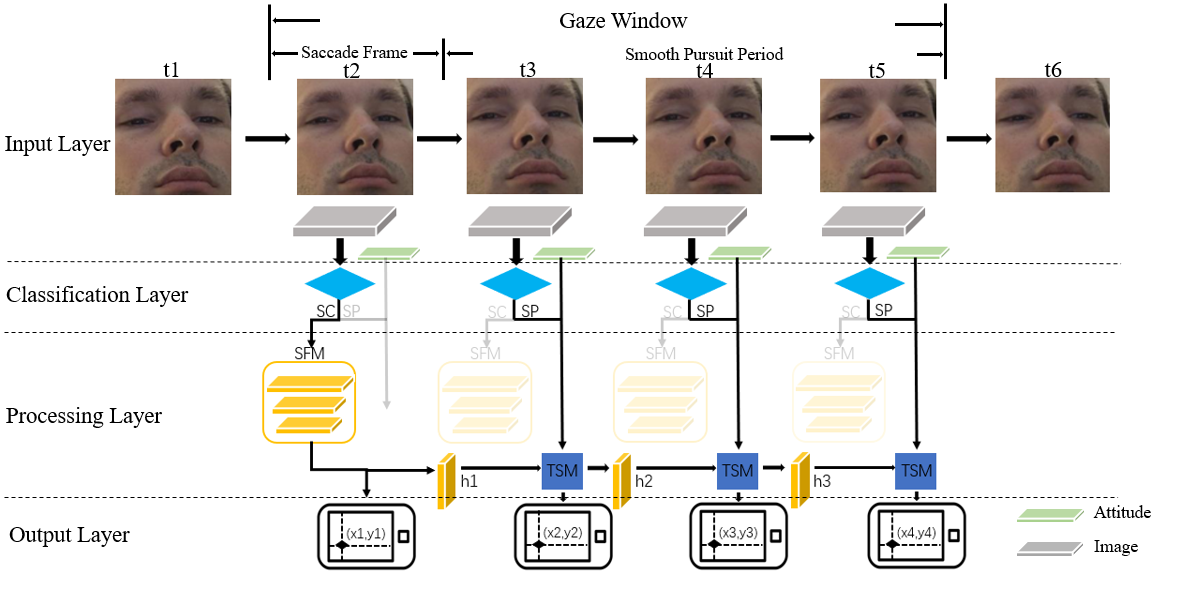
\includegraphics[scale=0.5]{pictures/time_flow_2.jpg}
  \caption{Time Series Architecture of GazeDance. t2-t5 exhibits a gaze window including an initial saccade frame and a following smooth pursuit period when the user gazes at a specific stimulus(note the gaze transformation between t1-t2 and t5-t6). The attitude of mobile devices and the image from the front camera are taken as the input of GazeDance. In the classification layer, the eye movement is classified as SC(saccades) and SP(smooth pursuit), for which the processing layer takes different strategies to process: SFM(single-frame model) for saccades and TSM(time-series model) for smooth pursuit. The two kinds of interframe information sharing are also reflected in processing layers as described in Sec. \ref{subsec:model_1}.}
  \Description{Time series data processing of GazeDance}
  \label{fig: time_flow}
\end{figure}

\section{GazeDance: Classification-based Eye-tracking System}
In this section, we describe GazeDance, the gaze-on-screen tracking architecture that achieves extreme efficiency as shown in Fig. \ref{fig: time_flow}. To adapt the eye-tracking model to the mobile scenarios with the limited computing power of devices and frequent jitters, we design a novel suspending mechanism through the transformation of interaction state. Subsection \ref{subsec:model_1} thoroughly demonstrates the suspending mechanism and explains how it could help build an efficient eye-tracking system, and Subsection \ref{subsec:model_2} makes a detailed introduction of the GazeDance system.

\begin{figure} 
  \centering
  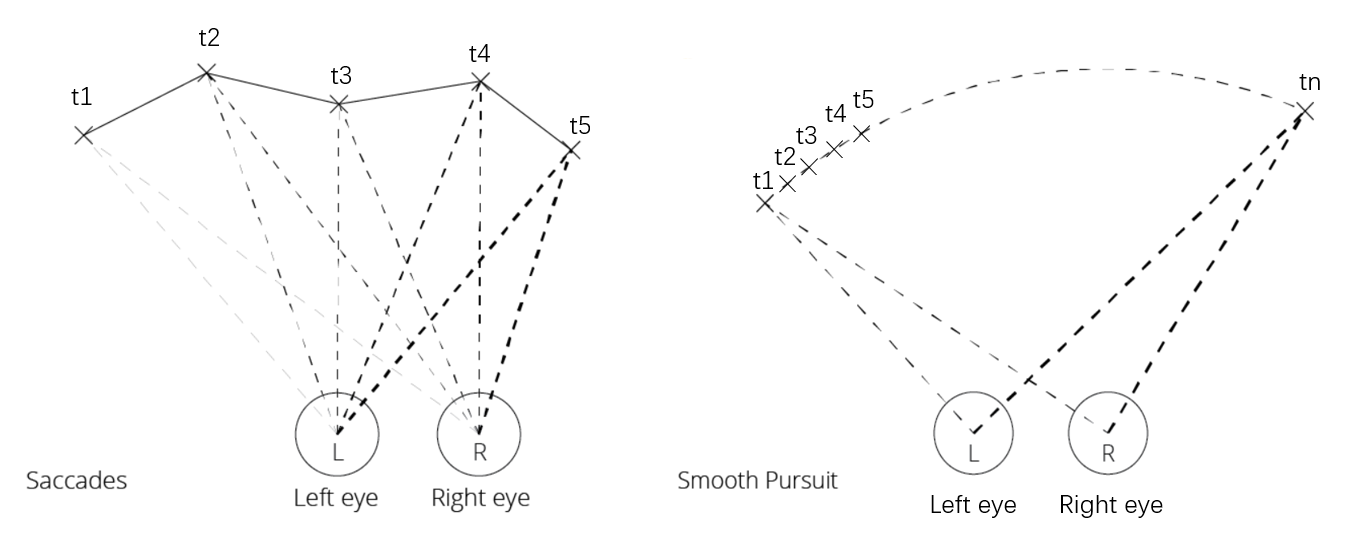
\includegraphics[scale=0.5]{pictures/types.png}
  \caption{Saccades and Smooth Pursuit}
  \Description{Saccades and Smooth Pursuit}
  \label{fig: eye movement}
\end{figure}

\subsection{Time-series Transformation Mechanism} \label{subsec:model_1}

% problems/research question
The last few years have seen the success of deep neural networks in appearance-based gaze-on-screen tracking task\cite{krafka2016eye,huang2017tabletgaze}. However, the complex pre-training and enormous computation in neural networks make it hard to get prompt feedback for mobile devices due to the limited resources such as battery life, processing speed, and bandwidth used compared to the computer cluster. It becomes a restriction of large-scale gaze-on-screen tracking applications. How to design a lightweight neural network specialized for mobile devices is proved to be a significant research question. 

%introduction of our model
Recently, eye movement analysis has become a popular topic for its high relevance to human-computer interaction such as understanding human emotion\cite{alghowinem2013eye} and interaction behavior\cite{lin2019eog}. However, little work has been put into an investigation about the correlation between eye movement and gaze estimation in spite of their essential biological connection. In this work, we manage to optimize the gaze-on-screen estimation model by leveraging eye movement biological characteristics. Specifically, we utilize the interframe relationship of different eye movement types and design a suspending mechanism with time-series eye movement transformation to simplify the gaze-on-screen problem.



%background
Generally speaking, the suspending mechanism is based on two characteristics of mobile gaze-on-screen interaction:

(1)The alternating of saccades and smooth pursuit. A saccade is a quick, simultaneous movement of both eyes between two or more phases of fixation in the same direction\cite{fuchs1967saccadic}, while smooth pursuit movements allow the eyes to closely follow a moving object instead of in jumps\cite{grasse1992analysis}as shown in Fig. \ref{fig: eye movement}. When observing static objectives such as reading a paper book, eyes do not move continuously along a line of text, but make short, rapid movements(saccades) intermingled with short stops(fixations)\cite{o1980control}. However, during mobile gaze-on-screen interaction in which jitter is inevitable and unneglectable\cite{peguero2016assessing}, the fixation interaction is replaced by smooth pursuit as the focusing point on-screen move with the mobile device. The alternating of saccades and smooth pursuit is the fundamental of taking different strategies for different interaction scenarios.

(2)The detectable state change. Firstly, saccades and smooth pursuit have a huge velocity difference. A saccade is one of the fastest movements produced by the human body and can reach up to a speed of 900 degrees/s\cite{fuchs1967saccadic}. In contrast, the smooth pursuit movement is relatively slow: the pursuit of targets moving with velocities of greater than 30 degrees/s tends to require catch-up saccades\cite{britannica1987sensory}. With the huge speed difference, the classification of eye movement can be easily built based on facial features. Further, the video capture rate of current mobile devices is high enough to detect the eye movement state change. Saccades last about 20–200 ms depending on their amplitude(20–30 ms is typical in language reading)\cite{afflerbach2015handbook}. For most mobile devices with a sampling interval of the same order of magnitude(~33 ms for 30 fps), the change of eye movement types could be easily captured as shown in fig \ref{fig: time_interval}.

\begin{figure} 
  \centering
  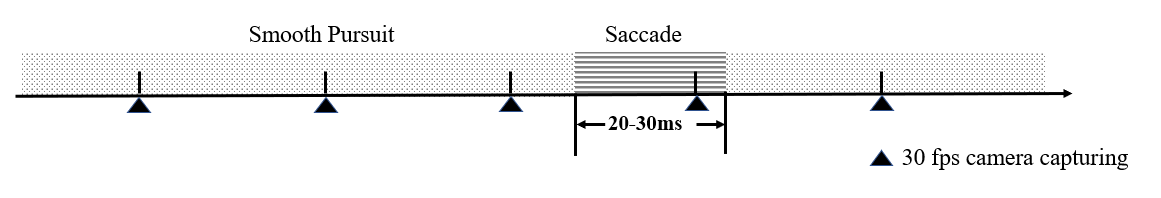
\includegraphics[scale=0.5]{pictures/time_interval.jpg}
  \caption{The lasting time of saccade and the interval of video record. With a camera capturing in 30 fps, the eye movement state could be easily captured by a mobile device.}
  \Description{a}
  \label{fig: time_interval}
\end{figure}

%mechanism
We introduce the suspending mechanism of GazeDance with time-series architecture as shown in fig \ref{fig: time_flow}. 
A gaze window including an initial saccade frame and a following smooth pursuit period is defined in the mechanism to represent the whole process of gazing at a specific stimulus. In general, two novel operations are leveraged in the mechanism: "divide-and-rule" and interframe information sharing.

(1) "Divide-and-rule". Benefit from the detectable state change, the eye movement classifier could be built simply on the changing scope between the last frame and the current moment, which guarantees the feasibility of division. Then, specialized estimation strategies of the two eye movement types are proposed on account of the distinction of saccades and smooth pursuit in tracking pattern: For smooth pursuit movements in which eye moves smoothly in a trackable pattern, GazeDance utilizes the correlation between the gaze prediction of consecutive frames. Specifically, we embed the time-series model in the gaze-on-screen tracking model for the first time. Further, the instant attitudes of mobile devices are also employed as data sources to eliminate jitter's impact on gaze prediction. With the information of image transmitting as the hidden state, GazeDance efficiently takes advantage of the tracking pattern of smooth pursuit to predict the gaze position instead of processing high-dimension image data. While for saccade with the simultaneous and elusory eye movement, no significant relationship between successive frames can be captured and we use a lightweight single-frame model to deal with this situation. 

(2) Interframe information sharing. As GazeDance utilizes a time-series model to process interframe relationship, how to transmit information between frames is an important question. We design two types of information sharing: sharing from saccades to smooth pursuit, and sharing between frames in smooth pursuit procedure. With the alternating of saccades and smooth pursuit\cite{Neuroscience2001}, there is strong continuity between the destination of a saccade and the origin of the following smooth pursuit in a gaze window. In this case, the hidden state of time-series model of smooth pursuit period is initialized to the last hidden layer of the single-frame model of the saccade, which is the first type of information sharing: the information sharing from saccades to smooth pursuit. While during smooth pursuit period, it is required to pass and update the tracking pattern. We keep the pattern in the hidden state of the time-series model, and it is the second sharing type: information sharing between frames in the smooth pursuit procedure.

% focus window

The time-series architecture in Fig \ref{fig: time_flow} could help better illustrate the suspending mechanism. $t_2$ to $t_5$ is a 4 frames wide gaze window. The frame at $t_2$ is classified as saccade because of the significant eye movement from the last frame, thus the gaze prediction is calculated by the single-frame model. At $t_3$ in which the user begins smooth pursuit, we initialize the hidden state of the time-series model with the last hidden layer of the single-frame model at $t_2$. That is to say, we share the information from saccades to smooth pursuit. $t_3$ to $t_5$ is a smooth pursuit period, and we share the tracking pattern information between frames through time-series model hidden state. For $t_6$ at which the user starts a new saccade, we stop the gaze window from moving forward and leverage the single-frame model to get gaze prediction again.


\begin{figure}
  \centering
  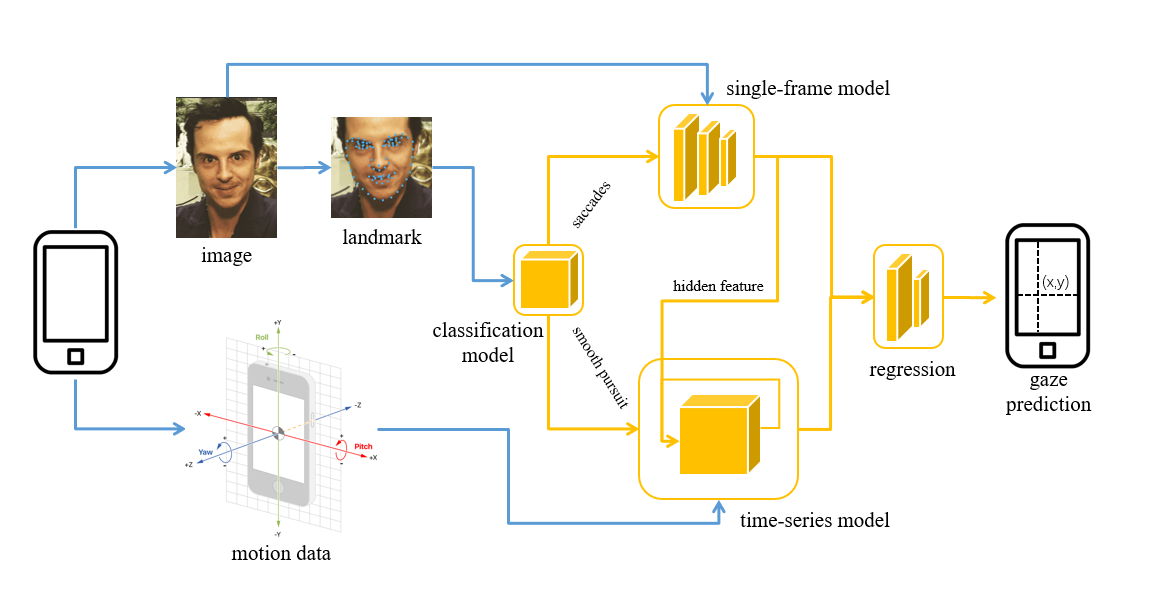
\includegraphics[scale=0.6]{pictures/architecture.jpg}
  \caption{Static Architecture of GazeDance}
  \Description{architecture}
  \label{fig:architecture}
\end{figure}

\subsection{Architecture}\label{subsec:model_2}
In this subsection, we will introduce the detailed design of each part of GazeDance architecture as shown in Fig. \ref{fig:architecture}. The architecture can be mainly divided into three components: classification, single-frame model for saccades and time-series model for smooth pursuit.

\textbf{Classification} \label{classification}
% (1) high performance under specific criteria, or it would only have a negative influence on the original framework;
% (2) low excess cost compared to the price of the whole model.

As an additional auxiliary layer, the classification model needs to satisfy both high performance and low cost. Seven features are selected per frame which could best demonstrate the eye-device relative movement as shown in Fig. \ref{eyeClassificationInput}: $(\Delta x,\Delta y)$ of pupil-to-corner displacement of two eyes separately(2*2) and $(\Delta Pitch, \Delta Roll, \Delta Yaw)$ of devices. To eliminate the impact of face size and rotation in the image, a specialized normalization strategy is designed for the eyeball movement. Without loss of generality, we take the right eye as the example to provide a detailed illustration. Firstly, $\Vec{a}$, the vector from left eye corner to right eye corner, is taken as the x-axis, and $\left| a \right|$ is defined as per unit length. In this reference system, we effectively avoid the influence of the inclination and zoom of the face in different real-world settings. Further, $\Vec{b}$, the vector from the left corner to the pupil, is utilized to calculate the eyeball movement with the following formula:

\begin{center}
\begin{math}
x = \frac{\vec a * \cos< \vec a, \vec b >}{\left| \vec b \right|} \quad
y = \frac{\vec a * \sin< \vec a, \vec b >}{\left| \vec b \right|}
\end{math}
\end{center}

As a continuous movement, the single frame information is not sufficient to make a robust prediction, thus we tune an appropriate sequence length of features in the experiment. A too-long sequence leads to a high-dimension input layer as well as much dirty data which has nothing to do with the current frame, while a too-small sequence length may have too few features to support a high-accuracy model. 

Note that for the two-class classification, we should pay more attention to avoiding a false negative result in which saccades are predicted as smooth pursuit. The reason is that compared to the false positive prediction(smooth pursuit predicted as saccades) which incorrectly takes the high-dimension single image as input and consequently reduces the processing time slightly, the false-negative prediction will have a severe impact on the accuracy of the whole model since the gaze of elusive saccades can not be easily caught by the movement trace. Under these circumstances, we choose recall instead of accuracy as criteria of the performance of the classification model.

\begin{figure}
  \centering
  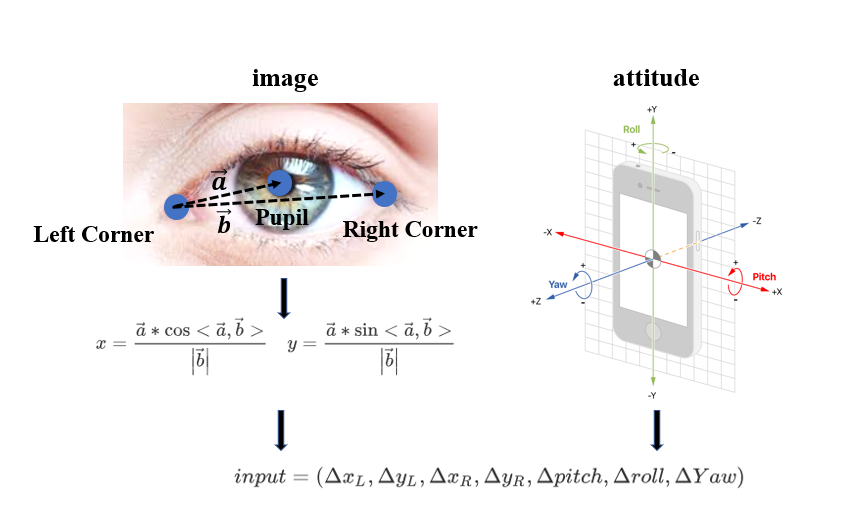
\includegraphics[scale=0.55]{pictures/eyeClassificationInput.jpg}
  \caption{eye classification features}
  \Description{eye classification features}
  \label{eyeClassificationInput}
\end{figure}

\textbf{Single-Frame Model for Saccades} \label{model:saccade}

The saccade phase is characterized by the fact that gaze points cannot be simply predicted based on the previous context. Therefore, the single-frame model needs to make the prediction based on the original single frame image captured by the front-end camera, which is the most common solution to the gaze-on-screen tasks.

% Based on the requirements of the GazeDance architecture, the single-frame model for saccades needs to satisfy the following two conditions: 
% 1. The single-frame model should be not only to serve as a component of GazeDance but also be a stand-alone module which could be integrated into any mobile application. Consequently, the convenient use of this component is required.

% 1. As explained in the suspending mechanism, the extracted features of the single-frame model will also be the input of the smooth pursuit component in addition to being the output of saccades, which raises a higher demand for accuracy.

% 2. As the most time-consuming of the three components, it will take a large proportion of the total processing time. Thus, speed is also a factor that can not be ignored.

Generally speaking, the single-frame gaze-on-screen task is similar to the facial point detection method to some extent with the same requirement of facial features especially eyes. At present, most of the facial point detection methods based on deep learning adopt the cascaded strategy \cite{sun2013deep, zhou2013extensive, zhang2016joint}. This is of great reference value to this work that cascade strategy can be considered as extracting facial or eye images to further predict gaze position, which hypothesizes that the gaze position is strongly related to eyes and the position of the face. Based on these, the feature is extracted in advance and input into the model separately. 

% The advantage of this method is that the model makes full use of priori knowledge and can get high-resolution local images. But for pre-processing part of extraction, integrating it into the independent model will increase processing time. If not, it will greatly increase the difficulty of other developers to use. That is to say, condition 1 and 3 cannot be satisfied at the same time.

Besides, according to ablation studies \cite{krafka2016eye}, what contributes to the gaze-on-screen prediction most are not high-resolution eye and face images, but the location information of the face. Therefore, the crux to designing a suitable single-frame model is to determine a method that can extract the location information directly from the original image and to meet our precision and time requirements. It needs to be a lightweight model with excellent performance, which can obtain better performance with fewer parameters.

Considering the conditions mentioned above, the single-frame model of GazeDance adopts MobileNetV2 \cite{sandler2018mobilenetv2} as the backbone, which is a convolutional neural network model for mobile devices designed to leverage residual ideas based on MobileNet. As a lightweight and efficient model, it perfectly satisfies the need to be deployed on mobile terminals with little loss of the ability of location information detection.

\textbf{Time-Series Model for Smooth Pursuit} \label{smooth}

The time-series model for smooth pursuit is the core component to improve computational efficiency and jitter adaptability of GazeDance by sharing interframe information in a flexible way, which is required to reduce the input dimension for the neural network as much as possible with little loss of tracking pattern information. Thus, this component takes (1)the instant attitude of mobile phone collected by the mobile motion sensor as input, and passes (2)gaze prediction information(included in the last hidden layer of the model of previous frames) as interframe information. We provide the theoretical basis of the selection of input data in this section. 

To simplify the problem, we generalize all kinds of low-speed relative movement between eye and screen (including relative stationary state) as "smooth pursuit". For the relative stationary state, gaze prediction remains the same as the previous result and can be easily calculated by a simple neural network. When a relative movement between eye and screen occurs, there are three kinds of gaze movement on the screen including: (1)the gaze movement caused by translational motion of eyes or mobile device, like reading a line of text on the screen; (2)the gaze movement caused by the rotation of mobile device, like shake; (3)the gaze movement with both translational motion and rotation, like the jitter of mobile device. We only discuss the first two cases for the reason that though the third case occurs most frequently, it can be seen as the synthesis of the first two cases.

For the first case when the gaze movement is caused by translational motion of eyes or mobile device, we can leverage the gaze prediction of several frames before the current moment to track the gaze motion trace. The gaze motion trace can be different at shape(anomaly, arc or approximately linear shape), acceleration(uniform acceleration and variable acceleration) and so on. To begin with, we try to solve the problem of uniform linear gaze motion. In most cases, approximately uniform linear motion makes up the majority of smooth pursuit. As shown in Fig. \ref{translational} left, the distance between gaze(t-3) and gaze(t-2) equals the distance between gaze(t-2) and gaze(t-1),  whose trace can be concluded as:

\begin{center}
\begin{math}
IF \qquad \Delta x_{g_{(t-2)}} == \Delta x_{g_{(t-1)}} \quad and \quad \Delta y_{g_{(t-2)}} == \Delta y_{g_{(t-1)}} \\
THEN  \quad y = y_{g_{(t-1)}} + \Delta y_{g_{(t-1)}}\quad and \quad x = x_{g_{(t-1)}} + \Delta x_{g_{(t-1)}}
\end{math}
\end{center}

\begin{figure}
  \centering
  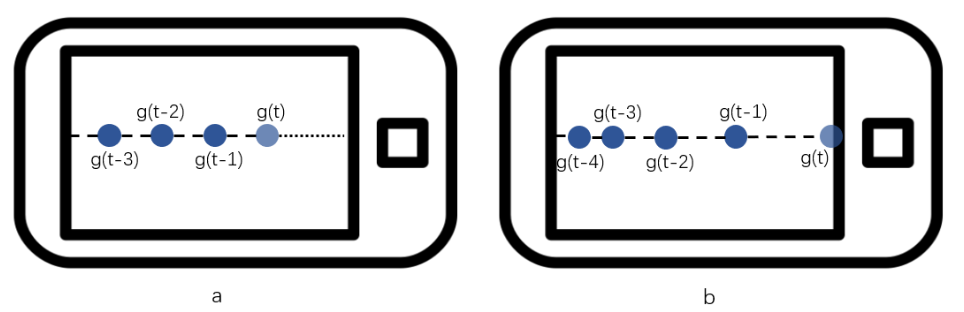
\includegraphics[scale=0.4]{pictures/slide_model.png}
  \caption{translational motion}
  \Description{translational motion}
  \label{translational}
\end{figure}

Fig. \ref{translational} right exhibits a more complicated case of linear gaze motion with uniform acceleration. Since the acceleration is not changed, this kind of trace can be described as:

\begin{center}
\begin{math}
IF \qquad \Delta x_{g_{(t-2)}} - \Delta x_{g_{(t-3)}} == \Delta x_{g_{(t-1)}} - \Delta x_{g_{(t-2)}} \quad and \quad \Delta y_{g_{(t-2)}} - \Delta y_{g_{(t-3)}} == \Delta y_{g_{(t-1)}} - \Delta y_{g_{(t-2)}} \newline
THEN  \quad y = y_{g_{(t-1)}} + \Delta y_{g_{(t-1)}} + (\Delta y_{g_{(t-1)}} - \Delta y_{g_{(t-2)}})\quad and \quad x = x_{g_{(t-1)}} + \Delta x_{g_{(t-1)}} +(\Delta x_{g_{(t-1)}} - \Delta x_{g_{(t-2)}})
\end{math}
\end{center}

Here, we prove that both traces can be easily learned by a recurrent neural network like GRU. Since the uniform linear gaze motion is a special case of uniform-acceleration linear gaze motion, we only discuss the latter. GRU cell can be represented as:

\begin{equation}
\begin{aligned}
X &= [x^t,h^{t-1}]\\
r &= sigmoid(W^rX+b^r)\\
z &= sigmoid(W^zX+b^z)\\
h^{t-1^{'}} &= h^{t-1}\odot r\\
X^{'} &= [x^t,h^{t-1^{'}}]\\
h^{'} &=tanh(W^hX^{'}+b^h)\\
h^t &= z \odot h^{t-1} + (1-z) \odot h^{'}
\end{aligned}
\end{equation}

in which hidden state $h^{t-1}$ contains time-series information with variable sequence length. We assume $h^{t-1}$is a linear representation of $\Delta y_{g_{(t-1)}}, \Delta y_{g_{(t-2)}}, \Delta y_{g_{(t-3)}}, \Delta x_{g_{(t-1)}}, \Delta x_{g_{(t-2)}}, \Delta x_{g_{(t-3)}}$. With $x^t$ including both $y_{g_{(t-1)}}$ and $x_{g_{(t-1)}}$,  $W^h$ matrix can easily learn the linear prediction:

\begin{equation}
\begin{aligned}
\quad y &= y_{g_{(t-1)}} + \Delta y_{g_{(t-1)}} + (\Delta y_{g_{(t-1)}} - \Delta y_{g_{(t-2)}})\quad \\
x &= x_{g_{(t-1)}} + \Delta x_{g_{(t-1)}} +(\Delta x_{g_{(t-1)}} - \Delta x_{g_{(t-2)}})
\end{aligned}
\end{equation}

With the help of intermediate state of GRU cell, $h^t$ can also be restored as the same linear representation of   $\Delta y_{g_{(t)}}, \Delta y_{g_{(t-1)}}, \Delta y_{g_{(t-2)}}, \Delta x_{g_{(t)}}, \Delta x_{g_{(t-1)}}, \Delta x_{g_{(t-2)}}$.  The relationship between adjacent predictions can move forward in this pattern.

For the second case when the gaze movement is caused by the rotation of the mobile device, the attitude of mobile devices plays a significant rule. As the simple example shows in Fig. \ref{rotation}, when the mobile phone rolls $\theta$ degrees to be perpendicular to the line of sight, the gaze point moves $L - Lsin\theta$. But in the mobile scenario in which three kinds of attitude \textit{roll, yaw, and pitch} often work together, the gaze trace brought by device rotation is complex and can not be well predicted by gaze sequence. The slight but frequent occurrence of rotation-brought gaze movements like jitter makes the problem unable to be neglected. Therefore, we also take the motion captured by the mobile sensor as input.

\begin{figure}
  \centering
  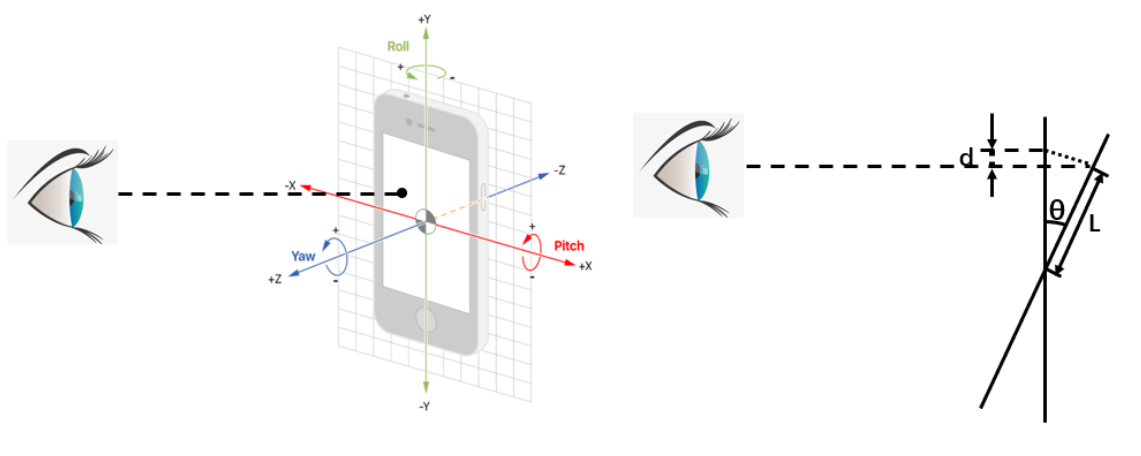
\includegraphics[scale=0.4]{pictures/rotation_model.png}
  \caption{rotation}
  \Description{rotation}
  \label{rotation}
\end{figure}


% dimensions:
% 0. across devices
% 1. compared to other algorithms
% 2. time and precision
% 3. time for different parts

\section{Experiment}
In this section, we make a thorough evaluation of the performance of GazeDance in real-world settings across multiple types of mobile devices. Overall, GazeDance significantly outperforms previous state-of-the-art approaches, achieving 6× speedup compared to the previous model with accuracy improvement by 15\% in the most generalized scenarios. We also sifted out some special cases and explored the context behind them.

\subsection{Experimental Scenario}\label{subsec:experiment scenario}

\textbf{Data preparation:} From 1,490,959 valid frames in GazeCapture with face and eye detections, we further exclude 32751 frames with abnormal records in terms of time or motion. We divide the dataset into train, validation, and test in the same way as iTracker for a fair comparison. Before training the model, the dataset is preprocessed by central cropping and resized to 224 * 224 pixels to accelerate the training speed.

Besides, a focus window of eye moving is defined: the first frame belongs to saccades, and all the remaining frames belong to smooth pursuit. The initial window partition can be divided according to screen dot, that is, all frames of one dot on the screen are divided into one window. This ensures that the first frame is determined to belong to saccades, but it does not guarantee that there are no saccades in the remaining frames. At this point, we can focus on the recall of classification described in section \ref{smooth}. The classification model is trained based on this and re-divide it iteratively.
    
Further, the motion data are required by the time-series model as described in section \ref{smooth}. It records at 60Hz which is much higher than the frequency of image acquisition. As a result, image and action data do not correspond to each other completely. We did the nearest point approximation pre-processing.

% \textbf{Implementation details:} The entire model was implemented using PyTorch \cite{paszke2017automatic}. We adopted the strategy of training each component separately, so some training details can refer to the corresponding sections of each component. 

%mark2: device

\textbf{Evaluation metric:} In terms of error, we reported Euclidean distances for predicted and actual positions. In terms of time, we only calculated the inference time of models, excluding the time to prepare the input data. Besides, unlike \cite{krafka2016eye}, we did not augment dataset, especially in the test phase. Their results were averaged on multiple augmenting the datasets, which took much more time and was unacceptable on the mobile side.

The main purpose here is to evaluate the generalization performance of the entire model, GazeDance, in the scenario without knowing device size, distance, and calibration, which can be considered as the worst-case of screen-to-face tasks.

We performed training using a Dell PowerEdge T640 server containing two Intel Xeon Silver 4110 2.10GHz 8-core processors, 64 GB of RAM, and four NVIDIA TITAN V GPUs and testing using multiple types of mobile devices including iPhone X, iPhone Xs Max, iPad Pro 11, Pixel 2, and Pixel 3.

\begin{table}
  \caption{Performance of Classification}
  \label{tab:classification}
  \begin{tabular}{lcccc}
    \toprule
    Model & Seq Length & Precision & Recall & Processing time(ms) \\
    \midrule
    SVM & 5 & 77.30\% & 77.30\% & - \\
    Random Forest & 5 & 77.30\% & 86.71\% & - \\
    \hline
     & 2 & 79.12\% & \textbf{94.99} \% & \textbf{1.34}\\
    XGBoost & 3 & 80.71\% & 94.30\% & 1.45\\
     & 5 & 82.71\% & 94.59\% & 1.57\\
    \hline
     & 2 & 98.00\% & 92.29\% & 3.20 \\
    GRU & 3 & \textbf{98.26}\% & 94.21\% & 3.19 \\
     & 5 & 97.99\% & 90.52\% & 3.20 \\
  \bottomrule
\end{tabular}
\end{table}

%GRU: note


\subsection{"DIVIDE": Eye Movement Classification}
As described in Sec. \ref{subsec:model_1}, the performance of eye movement classification determines the performance of the whole architecture. Data preparation in Sec. \ref{subsec:experiment scenario} provides the ground truth of eye movement types for gaze windows: the first frame of fixation at one dot is classified as saccades for the significant movement from the last dot, and the remaining frames belong to smooth pursuit because of the relatively smooth movement between eyes and mobile device. To reduce the cost at classification layers, we select seven features per frame which could best describe the eye-device relative movement as introduces in Sec. \ref{classification}: $(\delta x,\delta y)$ of pupil-to-corner displacement of two eyes separately(2*2) and $(\delta Pitch, \delta Roll, \delta Yaw)$ of devices. We evaluate the classification performance across different models(SVM, Random Forest, XGBoost and GRU) and sequence length(2, 3 and 5). The results are shown in Tab. \ref{tab:classification}. XGBoost\cite{chen2016xgboost} with 2 frames each sequence is ultimately selected for classification layer in consideration of both recall(94.99\%) and processing time(1.34ms). The classification model is further embedded into GazeDance System and tested in mobile scenarios.

% \begin{table}
%   \caption{Performance of single frame component of GazeDance}
%   \label{tab:backbone}
%   \begin{tabular}{lccc}
%     \toprule
%     Model & Params(M) & Time(ms) & Error(cm) \\
%     \midrule
%     iTracker & 6.29 & 84.15 & 3.33 \\
%     ResNet-50 & 0 & 0 & 0 \\
%     MobileNetV2 & 2.39 & 38.21 & 2.64 \\
%   \bottomrule
% \end{tabular}
% \end{table}

% calculate the errors according to the dot error method mentioned in the article for stream of frames. When calculating the average, we simulated the real scene, including only the data before the current time at the same fixation point.

\subsection{"RULE": Gaze Prediction} 

This section starts with the saccade case and then presents the implementation and performance of integrating smooth pursuit.

\begin{table}
  \caption{Performance of GazeDance: Experimental Environment on PC. The result of iTracker \cite{krafka2016eye} is derived by using its pre-training model and open-source implementation of PyTorch in the same environment. }
  \label{tab:gazedance}
  \begin{tabular}{llcc}
    \toprule
    Model & Remarks & Time(ms) & Error(cm) \\
    \midrule
    baseline & only saccade frames are calculated & 8.87 & 2.78 \\
    % iTracker & - & 6.29 & 84.15 & 3.33 \\
    iTracker* & dot error & 84.15 & 3.16\\
    Single-frame & all frames by single-frame model & 38.21 &\textbf{ 2.64} \\
    GazeDance & "divide-and-rule" & \textbf{9.58} & 2.68 \\
  \bottomrule
\end{tabular}
\end{table}

\textbf{Saccade: single-frame model.} \label{subsec:backbone}
According to the discussion in the Sec. \ref{model:saccade}, the original image containing location information serves as a data source for the end-to-end single-frame model. MobileNetV2 is chosen as a backbone to extract information from those images, for its excellent precision and speed balance on mobile devices.

Firstly, in order to keep the consistency of the relative position of different image sizes, we adopt the central crop method to process the original image rather than resizing. Since the position of the face is critical to the gaze position, any unequal scaling is unacceptable. 

The original MobileNetV2 was designed for classification, so we replaced their last layer with two full connection layers(with sizes: FC1: 128, FC2: 2) without activation function for regression shown in the regression part in Fig. \ref{fig:architecture}. The final output is x, y coordinates so it can also be used as a model-independent plug-in, which can be easily deployed to any mobile application independently.

The model uses Adam \cite{kingma2014adam} as the adaptive gradient optimizer with Euclidean distance as the loss function. Lr starts at 0.1 and decays to 1/10 of the previous epoch in the second and tenth epochs. Except for the last regression part, other layers were pre-trained on ImageNet \cite{deng2009imagenet}.

In the evaluation, the single-frame model was applied to every frame on the test set, not only the saccade phase. By contrast, in a gaze window, only the saccade frame was calculated, while the rest is filled with this result. The latter is regarded as our baseline model. As for the baseline model, the test set is partitioned into sequences according to the fixation points.

The results are shown in Tab. \ref{tab:gazedance}. Both time and error are the average values of test datasets. Interestingly, we find that the baseline model outperforms the former state-of-the-art approaches despite none of the subsequent frames were computed. It shows that the saccades phase of our single-frame model can extract the eyes and location context from the original image very well. Considering that this test dataset mixes all the different screen sizes including devices like the iPhone and the iPad and all four orientations, which far more complicated than the actual use, this is a surprising result. At this phase alone, it has surpassed the previous model both in accuracy and speed. 

\textbf{Smooth pursuit: time-series model}
For the time-series model backbone, we choose GRU specifically for its high efficiency and brief structure which proved in Chap. \ref{smooth}. Features of the nearest saccade frame extracted by the single-frame model are used to initialize the hidden-state. Subsequent frames only take motion sensor data as input.

When put into practice in mobile scenarios, the time-series model shows its advantages as follows: (1)High efficiency. Compared to an image composed of numerous pixels, the input of the time-series model significantly decreases. It reduces not only the model processing time but the IO cost as well, which is crucial to mobile scenarios. (2)Low energy consumption. The small number of parameters in this model ensures a low energy cost and a small storage requirement. (3)The availability for higher accuracy demand. Compared to images captured by the mobile camera, the motion data collected by mobile sensors can have a much higher frequency. Low-frequency image collection might be a restrict of eye-tracking when designing a higher accuracy model in the future, while using motion data can solve this problem to some extent. Note that people tend to perform smooth pursuit more than saccades in most mobile tasks, so the performance of the smooth pursuit model can have a higher influence on the whole model. 

All those results are shown in the Tab. \ref{tab:gazedance}. Compared with the baseline, the error is reduced by 0.1cm, which proves the effectiveness of the time-series model. Its accuracy is not as good as the pure single-frame model, which is expected considering only a quarter of reasoning time consumed. Overall, GazeDance achieves the best balance between accuracy and speed.

% Importantly, we recognize that this is only effective in the case of fixed-point tasks in dataset acquisition, and there is no such scenario in real life. Therefore, excluding the baseline model, 

\begin{figure}
  \centering
  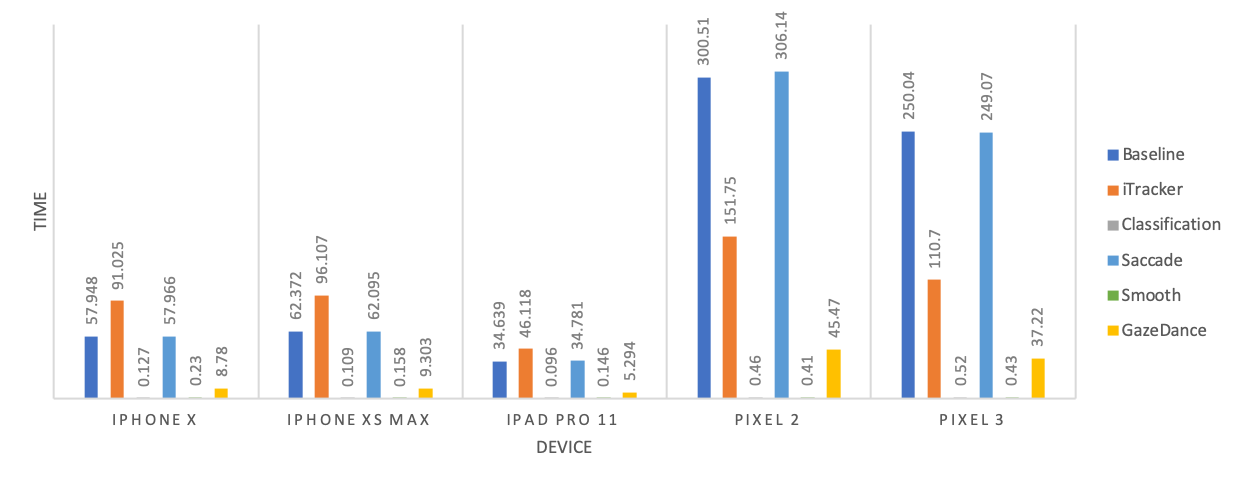
\includegraphics[scale=0.8]{pictures/time_platforms.png}
  \caption{Comparison under Mobile Scenario}
  \Description{Comparison under Mobile Scenario}
  \label{fig:time_platforms}
\end{figure}

\subsection{Mobile Scenario}

In this section, we evaluate the efficiency of several models including the single-frame model and GazeDance in mobile scenarios. The model needs to be transformed into an adaptive form with a mobile framework that can be deployed on iOS and Android operating systems. Our model is implemented by PyTorch, and we naturally chose PyTorch Mobile as the mobile deployment framework. In addition, in order to fully obtain the performance of iOS devices, we take Apple's exclusive Core ML platform into account. Right legend of Fig. \ref{fig:time_platforms} shows the six environments we used for our evaluation. The models were not trimmed during the conversion process, so the error is the same as on the PC platform, which will not be listed additionally here. 

% \begin{table}
%   \caption{Performance of GazeDance on multiple platforms}
%   \label{tab:devices}
%   \begin{tabular}{llccc}
%     \toprule
%     No. & Device & System & Framework & Time(ms) \\
%     \midrule
%     1 & iPhone X & iOS 13 & Core ML 3 & 0 \\
%     2 & iPhone X & iOS 13 & PyTorch Mobile & 0 \\
%     3 & iPad Pro 11 & iPadOS 13 & Core ML 3 & 0 \\
%     4 & iPad Pro 11 & iPadOS 13 & PyTorch Mobile & 0 \\
%     5 & Pixel 2 & Android 8 & PyTorch Mobile & 0 \\
%     6 & Pixel 3 & Android 9 & PyTorch Mobile & 0 \\
%   \bottomrule
% \end{tabular}
% \end{table}

Fig. \ref{fig:time_platforms} shows that GazeDance still has obvious speed advantages on various platforms in the mobile scene, achieving ∼6× speedup compared to previous work. In terms of time, GazeDance is currently affordable on common mobile devices.


\subsection{Case Study} \label{analy}
In practical mobile applications, features exhibited in different scenarios have different impacts on model performance. To figure out the influence factors, we make a case study by manually coding 1000 badly-performed images with error greater than 5cm and 1000 well-performed images with error less than 1cm. Two types of prediction error are concluded here: error caused by eye/face feature missing and error caused by inaccurate detection. Then, we discuss the good performance for the slightly blurred image which is commonly believed problematic and explores the reasons behind it. 

\begin{figure} 
  \centering
  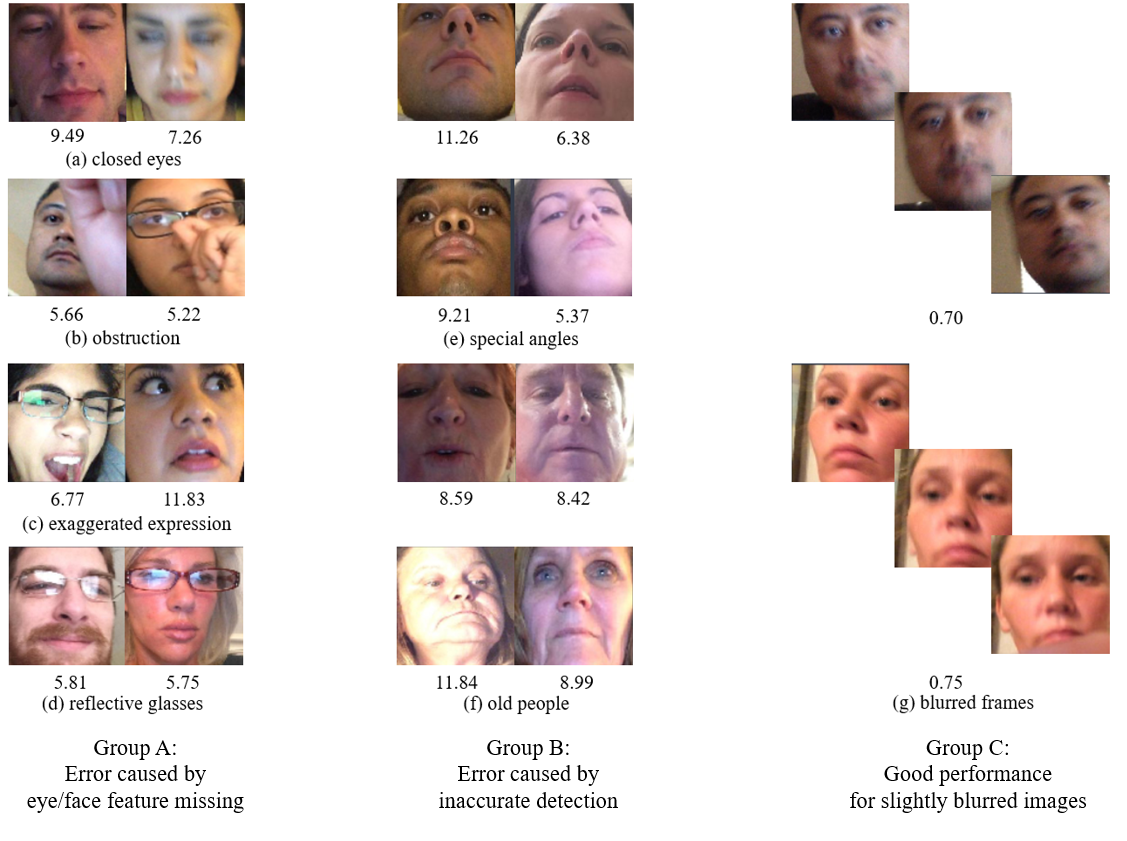
\includegraphics[scale=0.5]{pictures/analysis.jpg}
  \caption{Special case analysis. The numbers below pictures are the corresponding prediction error(cm) for Group A and B, and the average prediction error(cm) in the sequence for Group C.}
  \Description{special case analysis}
  \label{fourtp}
\end{figure}

The most typical badly-performed scenarios directly hinder the face feature detection and thus reduce the precision such as \textbf{closed eyes, obstructions, exaggerated expression, and reflective glasses} as Group A of Fig. \ref{fourtp} shows. In particular, when eye features are hidden, the model performance would be affected severely because of the influence on every stage of GazeDance. 


We also find two scenarios in which the whole face features could be found but the model still performs badly. The first one is related to \textbf{old people} shown in case(f) of Fig. \ref{fourtp}. It is noticed that 79 characters in 1000 badly-performed images were old people, whose rate is three times higher than the normal samples we observed. Two possible explanations are raised for this phenomenon:(1)Wrinkles may interfere with landmark recognition. (2)Thick eyelids may affect the judge of eye features. The second scenario is about \textbf{special angle}. An important feature of the mobile-camera image is the bottom-up angle as shown in case(e) of Fig. \ref{fourtp}. It could result in image distortion, which causes the landmark detection error.


A common belief is that the \textbf{blurred image} could lead to a huge error in the eye-tracking task. However, we found that most of the slightly blurred image had a not bad performance in gaze-to-screen tracking, as Group C in Fig. \ref{fourtp} shows. A hypothesis is that the interframe information sharing during smooth pursuit period can save transient "memory" of gaze prediction, which improves the jitter adaptability of GazeDance system.

\section{application}

In this section, we developed a simple eye tracking app based on GazeDance and demonstrate the advantage of delay in fast moving scene.

We also showed another case of attaching the mobile device running this app to other devices as a tracker. It can be easily embedded into existing research applications and allows designers and researchers to focus on the interaction concepts instead of the complex implementation.

\subsection{tracking delay}

The accuracy of GazeDance has been proved on large-scale and complex scene datasets. So the problem was simplified to a binary classification problem to eliminate the impact of tracking accuracy and focus on the delay.

In this app, a red circle shows up and down alternately on the screen at 10 Hz. Fig. \ref{fig:diagram} show the app's interface and tracking sequence diagram. As the sequence diagram shows, GazeDance tracked significantly more closely than the previous state-of-the-art model. The average delay of the two models is 19.7ms and 73.0ms respectively.

\begin{figure} 
  \centering
  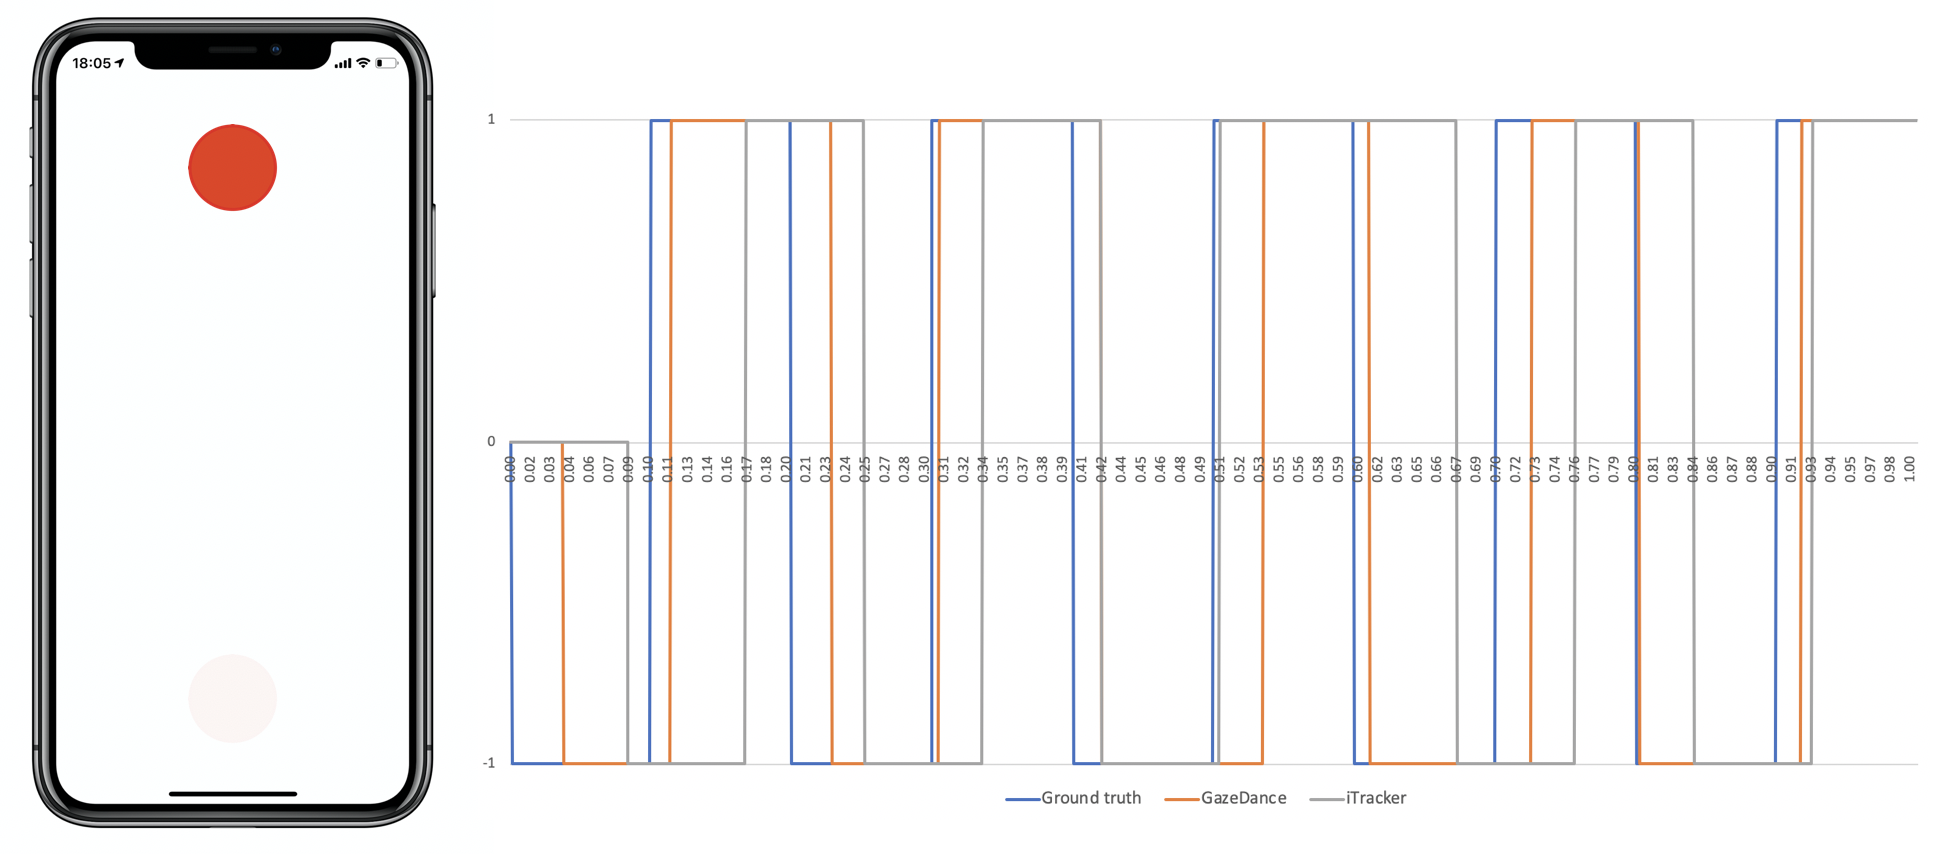
\includegraphics[scale=0.5]{pictures/device&diagram.png}
  \caption{The left part is the tracking app, and the red circle is displayed alternately at the top or bottom(transparent) position. The right part is the sequence diagram. The horizontal axis is the time axis. The vertical axis 1 represents the top and - 1 represents the bottom position}
  \Description{}
  \label{fig:diagram}
\end{figure}

% \subsection{As a tracker for HFR games}


\section{Conclusion}
In this work, we introduce GazeDance, a high-performance gaze-on-screen tracking model specialized for mobile devices. To optimize the enormous computation problem of neural networks and lower the impact of jitter during mobile use, a novel suspending mechanism is designed with two core strategies: "divide-and-rule" and interframe information sharing. GazeDance reduces processing time per frame of gaze prediction to 37.22ms, 8.78ms and 5.29ms for Pixel 3, iPhone X and iPad Pro, achieving ∼6× actual speedup compared to the previous model in the same environment while improving the accuracy by 15\%. GazeDance has been further expanded into an open-source industrial-strength toolkit for real-time gaze tracking, which could provide prompt interaction feedback for users and comprehensive statistical analysis for analysts or researchers. We hope our work can become an important step to bring high-performance gaze-on-screen tracking to everyday life.

\section{Limitation and Future works}
Limited to existing datasets, the circumstances of curve track is not included in this work - though it is not common except some special scenario like games. Seeing it from another angle, jitter also reflects the curve track to a certain extent in terms of relative motion.

A future direction of our work is to explore the eye movement type in different mobile tasks such as reading e-books, playing mobile games or chatting. We believe saccades and smooth pursuit proportions can differ a lot in different mobile tasks, which could help us design more specific models for them. Besides, to deeply figure out the influence of different problematic scenarios mentioned in \ref{analy} could be also a promising future work. 

% \section{Acknowledgments}


%%
%% The acknowledgments section is defined using the "acks" environment
%% (and NOT an unnumbered section). This ensures the proper
%% identification of the section in the article metadata, and the
%% consistent spelling of the heading.
% \begin{acks}
% To Robert, for the bagels and explaining CMYK and color spaces.
% \end{acks}

%%
%% The next two lines define the bibliography style to be used, and
%% the bibliography file.
\bibliographystyle{ACM-Reference-Format}
\bibliography{sample-base}

%%
%% If your work has an appendix, this is the place to put it.


\end{document}
\endinput
%%
%% End of file `sample-acmlarge.tex'.
